% PREAMBLE ------------------------------------------------------ {{{

\documentclass[12pt]{article}

\usepackage{amsmath,amsfonts,mathtools,graphicx,amssymb,dirtytalk}
\usepackage[margin=0.21in]{geometry}
\usepackage[]{microtype}
\graphicspath{{./3-img/}}
% using tikz, for Venn diagrams in this case
\usepackage{tikz}
% using tikz commands (must come after \usepackage{tikz})
% http://users.ju.edu/hduong/math220/venn_diagrams.pdf
\usetikzlibrary{shapes, backgrounds}

% binomial exponent
\newcommand{\negativeBinomial}[3][2]{(#2- #3)^{#1}}
% large math
\newcommand*{\largeMath}[1]{\mbox{\Large$#1$}}
% huge math
\newcommand*{\hugeMath}[1]{\mbox{\huge$#1$}}

%}}}
\begin{document}
% SECTION: Set Notation and Operations -------------------------- {{{

\section*{Set Notation and Operations}

  % EXAMPLE DATASETS -------------------------------------------- {{{

  \paragraph{Example Datasets:}
  \begin{align*}
    X = \{3, 12, 9, 18, 21, 24\} && \text{AND} &&
    Y = \{12, 15, 6, 3, 9\}
  \end{align*}

  %}}}
  % SUBSECTION: Intersection of sets ---------------------------- {{{

  \subsection{Intersection of Sets: $X \cap Y$}
  \paragraph{Description:} An intersection contains elements that are in both sets. Can be thought of as \say{AND}.

  \begin{equation}
    X \cap Y = \{3, 12, 9\}
  \end{equation}%

  %}}}
  % SUBSECTION: Union of Sets ----------------------------------- {{{

  \subsection{Union of Sets: $X \cup Y$}
  \paragraph{Description:} A union contains elements that are in either set. Can be thought of as \say{OR}.

  \begin{equation}
    X \cup Y = \{3, 12, 9, 18, 21, 24, 15, 6\}
  \end{equation}%

  %}}}
  % SUBSECTION: Relative Complement / Set Difference ------------ {{{

  \subsection{Relative Complement or Difference between Sets: $X - Y$}
  \paragraph{Description:} Return a set with all the things in another set removed, or take out anything from one set that is in the other set(s). Also called the relative complement. Examples below show several ways to think about it and denote this. % chktex 36

  \begin{align}
    X - Y = \{18, 21, 24\} &&
    \text{\say{Y subtracted from X}} \\
    X \setminus Y = \{18, 21, 24\} &&
    \text{\say{Relative complement of Y in X}} \\
    Y - X = \{15, 6\} &&
    \text{\say{Elements of Y, with the elements of X removed}} \\
    Y \setminus X = \{15, 6\} &&
    \text{\say{Again, can be denoted as relative complement of X in Y}}
  \end{align}%

  \paragraph{Intuition:} What would the relative complement of set be if we complement it by itself?

  \begin{align}
    X - X = \{\} && \Rightarrow &&
    \text{\say{The result is the empty or null set. $\O$ or $\varnothing$}} \\
    X \setminus X = \{\} && \Rightarrow &&
    \text{\say{Every item is removed when it is complemented by itself.}}
  \end{align}%

  %}}}
  % SUBSECTION: Universal Set / Absolute Complement ------------- {{{

  \subsection{Universal Set ($U$) and Absolute Complement ($A'$) ($A\setminus$)}

  \paragraph{Description:}
  A universal set ($U$) is the collection of all objects in a particular context or theory. All other sets within this framework constitute a subset. In this case let A = a subset. So ($A'$) or ($A\setminus$) would be all the objects in the universe that is NOT in A.

  \begin{align}
  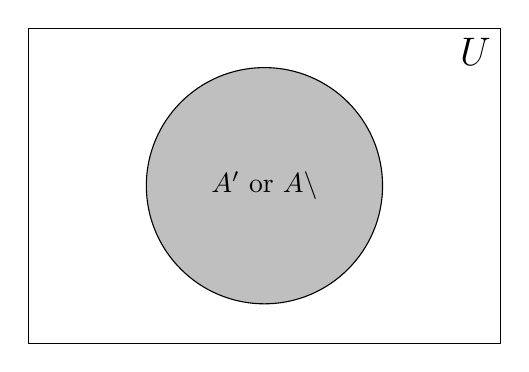
\begin{tikzpicture}
    \draw (-3,-2) rectangle (3,2) node[below left]{\largeMath{U}};
    \fill[lightgray] (0,0) circle (1.5cm) node {$A'$ or $A\setminus$};
    \draw (0,0) circle (1.5cm) node {$A'$ or $A\setminus$};
  \end{tikzpicture} && % chktex 31
  \begin{tikzpicture}
    \draw (-3,-2) rectangle (3,2) node[below left]{U=\mathbb{Z}};
    \fill[lightgray] (0,0) circle (1.5cm) node {C = {1, 2, 3}};
    \draw (0,0) circle (1.5cm)  node {C = \{1, 2, 3\}};
  \end{tikzpicture}
  \end{align}

  \paragraph{Example:}  $A' = (U - A) = (U\setminus A)$ and $C' = (U - C) = (U\setminus C)$, so $\{1, 2, 3\} \notin C'$.

  %}}}

%}}}
\end{document}
